% !TEX root = main.tex


\subsection{Outdoor PS conditioning}
\label{sec:sensitivity-analysis}

In the following, we consider a small planar surface patch with normal vector ${\bf n}$ and Lambertian reflectance with albedo~$\rho$. As discussed in~\cite{holdgeoffroy-iccp-15,hung-wacv-15}, the lighting contribution of an environment map to a Lambertian surface patch can be formulated as in an equivalent problem with a single point light source $\bar{\mathbf{l}} \in \mathbb{R}^3$. This vector is the mean of the light vectors computed over the hemisphere of incoming light directions defined by ${\bf n}$. This virtual point light source $\bar{\mathbf{l}}$ is henceforth referred to as the {\em mean light vector} (MLV). It is important to note that, as opposed to the traditional PS scenario where point light sources are fixed and thus independent of ${\bf n}$, here the {\em per-pixel} MLV is a function of $\mathbf{n}$. Thus, patches with different orientations define different sets of MLVs (as discussed later and shown in fig.~\ref{fig:realShiftNormal}).

Given multiple images of the same patch, taken at different times, we collect all photometric constraints for that patch and obtain the PS equation in matrix form:
%
\begin{equation}
\mathbf{b} =
\begin{bmatrix}
 b_1 \\ b_2 \\ \vdots \\ b_T
\end{bmatrix}
= 
\begin{bmatrix}
 {\bf \bar l}_1^T \\ {\bf \bar l}_2^T \\ \vdots \\ {\bf \bar l}_T^T
\end{bmatrix}
{\bf x} = \mathbf{L} \mathbf{x} \,,
\label{eqn:matrix-form}
\end{equation}
%
where $b_i \in \mathbb{R}$ are the observed pixel intensities, and ${\bf x} \in \mathbb{R}^3$ is the surface normal ${\bf n}$ scaled by $\rho$.

Let $\hat{{\bf x}}=({\bf L}^T{\bf L})^{-1}{\bf L}^T{\bf b}$ denote the least-squares solution of~\eqref{eqn:matrix-form}. A 95\% confidence interval for normal ${\bf x}$ is given by 
%
\begin{equation}
\hat{\mathbf{x}} \pm \bolddelta \,, \quad \text{with } \delta_k = 1.96 \frac{\sigma}{\rho}\lambda_k \,,
\label{eqn:confidence-xyz}
\end{equation}
%
where $\sigma$ is the camera noise level and $\lambda_k$ is the square root of the $k$-th element on the diagonal of $({\bf L}^T{\bf L})^{-1}$~\cite{hastie-book-09}. 

% A more intuitive measure of uncertainty in the estimate $\hat{{\bf n}}$ is obtained by considering angular distances $\theta$ in degrees, 
% % 
% \begin{equation}
% \theta^\pm = \cos^{-1}({\bf \hat n}^T{\bf \hat n}^\pm)\,, 
% \quad \text{where }
% {\bf \hat n}^\pm = \frac{{\bf \hat n} \pm \bolddelta}{\lVert{\bf \hat n} \pm \bolddelta \rVert}.
% \label{eqn:angular-dist}
% \end{equation}
% %
% Our measure of uncertainty, or stability, in the estimation of ${\bf \hat n}$ is then defined as the confidence interval \mbox{$\mathcal{C}_{\bf n} = [ 0, \max(\theta^\pm) ]$} in degrees.

% In the analysis below, we often take the estimate ${\bf \hat n}$ to be the ground truth normal ${\bf n}$ of a simulated (synthetic) surface patch; this corresponds to the result of an ideal algorithm. We then evaluate the confidence interval for this normal using a set of real, outdoor environment maps with associated stability parameters $\lambda_k$ as in~\eqref{eqn:confidence-xyz}. The result is a measure of the uncertainty in the reconstruction that an actual outdoor PS algorithm would provide on that particular set of illumination conditions, and surface orientation. As in~\cite{holdgeoffroy-iccp-15}, our simulations below consider synthetic surface patches with albedo $\rho = 1$ and a small, non-negligible noise level $\sigma$ at $1\%$ of the maximum pixel value.

From \eqref{eqn:confidence-xyz}, note that the only light-dependent stability factor in the confidence interval $\bolddelta$ is $\lambda_k$; the other two factors are related to the camera ($\sigma$), and surface reflectance~($\rho$). In this paper, we analyze the maximum uncertainty \mbox{$\lambda_\text{max} = \max_k(\lambda_k)$}, as a conservative performance measure that is independent of albedo and sensor noise; $\lambda_\text{max}$ is a {\em maximum noise gain} factor, \ie, the intensity of noise amplification in the solution. Here, we are interested in (\emph{i}) investigating how the noise gain $\lambda_\text{max}$ is influenced by the duration of outdoor data capture, and in (\emph{ii}) identifying specific changes, or {\em events}, in outdoor lighting that are associated with more stable PS solutions (smaller $\lambda_\text{max}$).

To make our analysis tractable, we do not model cast shadows and inter-reflections. In addition, we assume that the sky hemisphere (around zenith) provides the dominant part of incoming light. Unless stated otherwise, our simulations consider a day near an equinox, which corresponds to the worst case scenario with coplanar sun directions~\cite{shen-pg-14}.


\subsection{$x$-hour outdoor PS}
%\subsection{Time interval analysis}
\label{sec:analysis}

This section provides the first answers to the questions raised above by looking at collections of mean light vectors (MLVs) from both simulated and real sky data. The main goal is to analyze the behavior of the illumination factors $\lambda_k$ (and associated confidence interval) of normal estimation. More specifically, we investigate numerical stability (MLV coplanarity) as a function of the apparent sun motion and cloud coverage within capture intervals of different durations, containing different atmospheric events. We also compare the resulting performance measures of $x$-hour outdoor PS to those of full-day outdoor PS.

% Here our goal is to answer the questions: \emph{what} are the important changes, or {\em events}, in outdoor lighting that affect $\lambda_k$? What is the minimum duration of data capture, containing one or more of such events, that can lead to performance similar to that of full-day PS?

% -----------------------------------------------------------------------------
\begin{figure}[t]
\centering
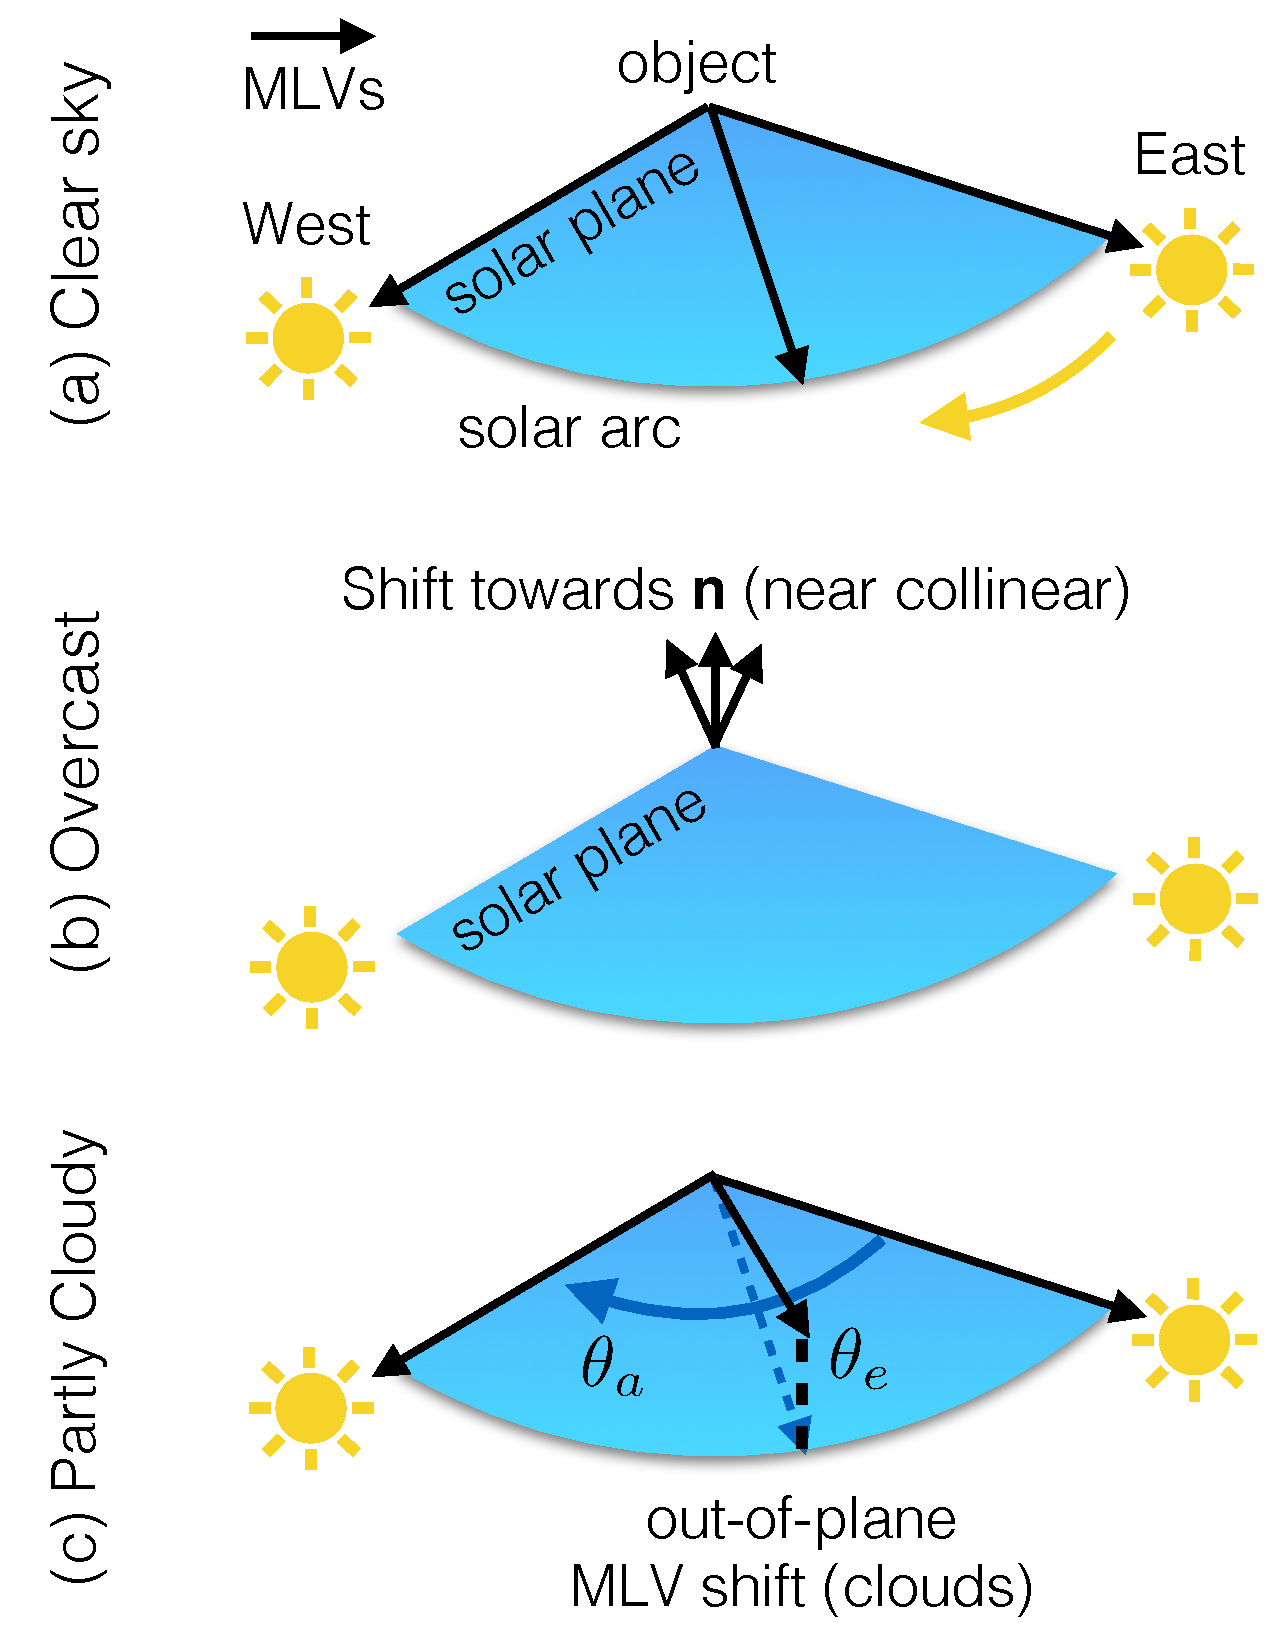
\includegraphics[width=.8\columnwidth]{diagram_MLVshift3}
\caption{Impact of cloud coverage on the numerical conditioning of outdoor PS: clear (a) and overcast (b) days present MLVs with stronger coplanarity; in partly cloudy days (c) the sun is often obscured by clouds, which may lead to out-of-plane shifts of MLVs.}
\label{fig:MLVshift}
\end{figure}
% -----------------------------------------------------------------------------
% -----------------------------------------------------------------------------
\begin{figure*}[t]
\centering
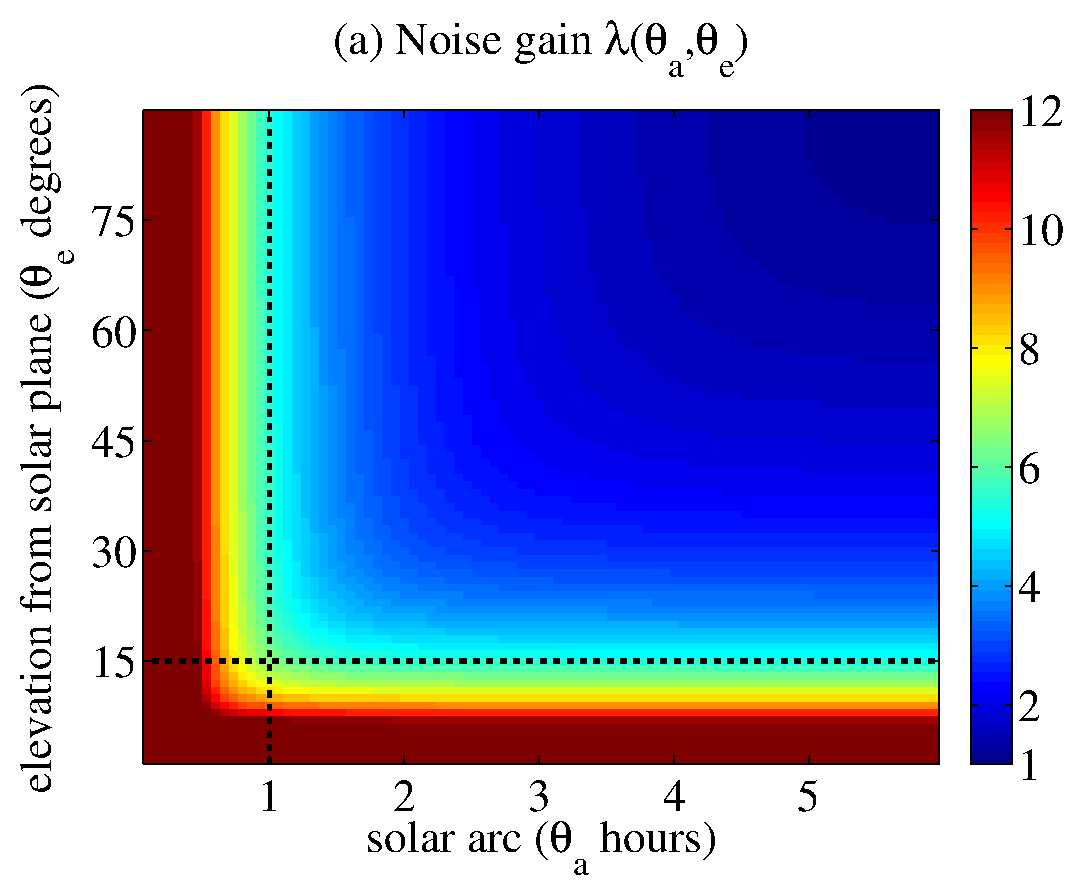
\includegraphics[width=.32\textwidth]{v123gainSurf} \ \ \ %\\[3mm]
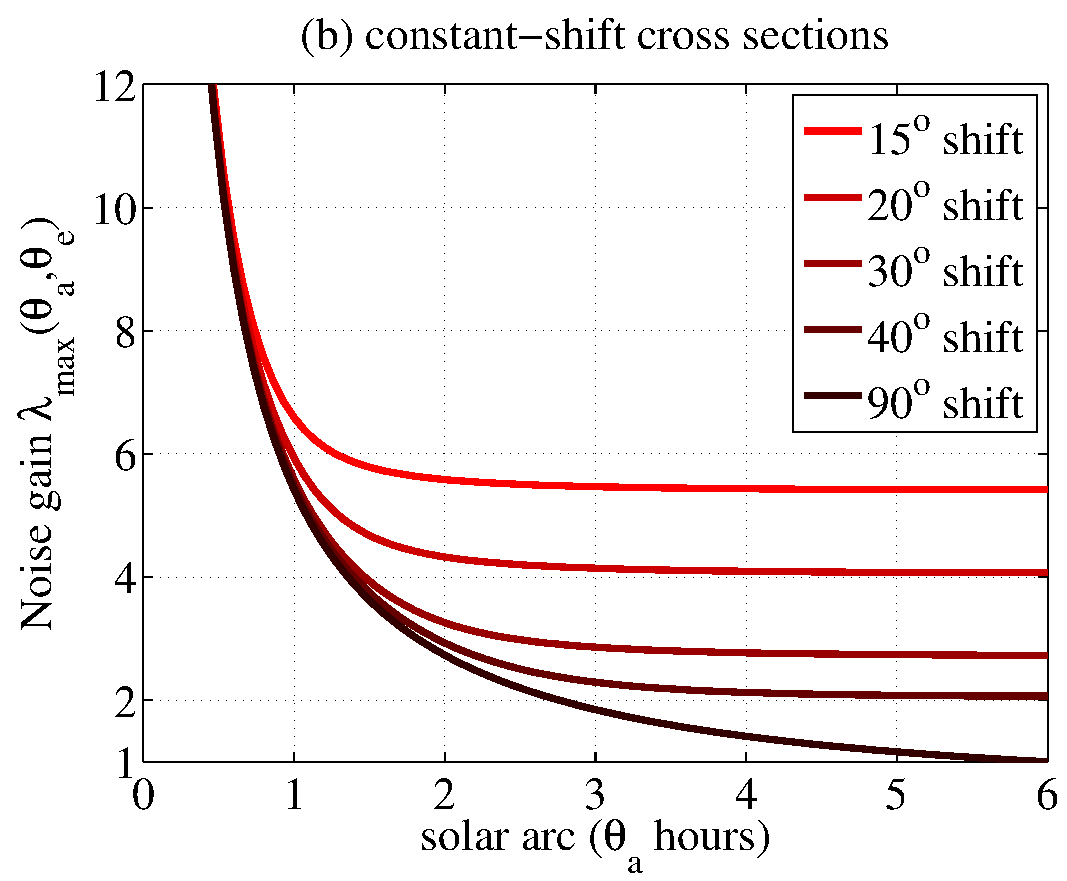
\includegraphics[width=.32\textwidth]{v123gain1Arc} \ \ \ %\\[3mm]
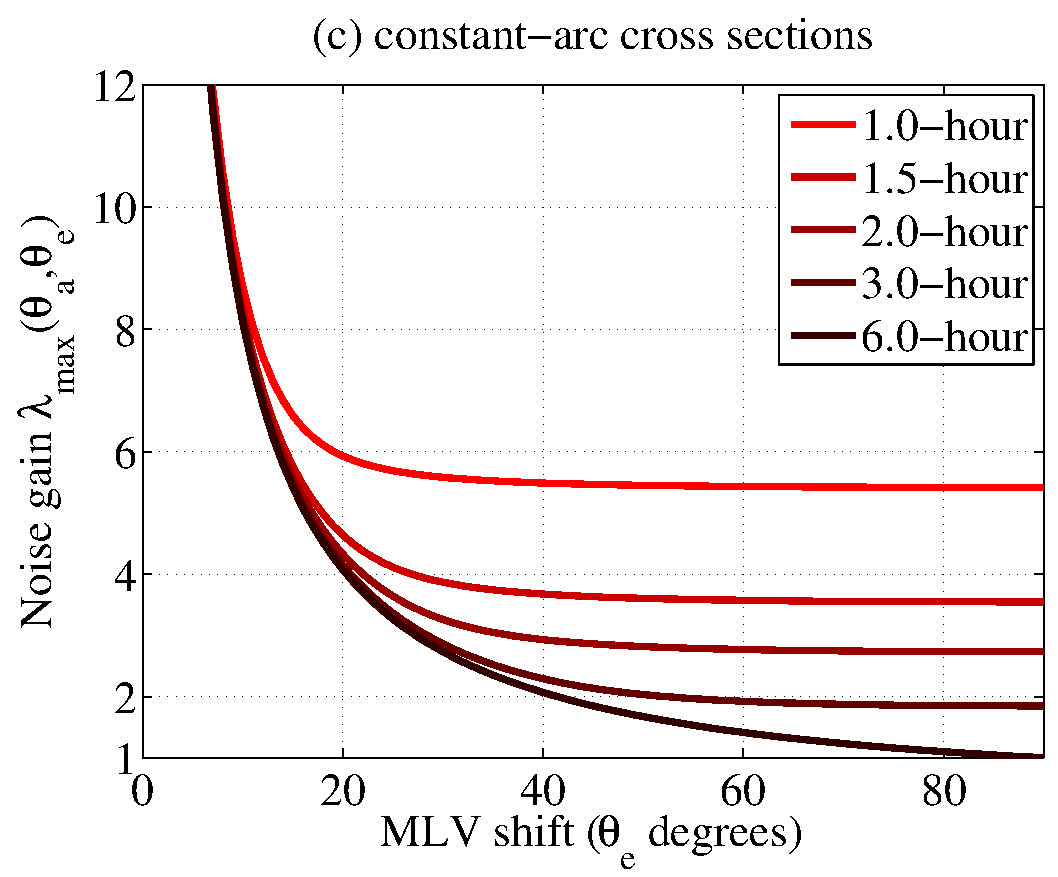
\includegraphics[width=.32\textwidth]{v123gain2Shift}
\caption{Simulated noise gain $\lambda_{\max}(\theta_a,\theta_e)$ as a function of solar arc $\theta_a$ and MLV shift (elevation) angle $\theta_e$. See discussion in the text.}
\label{fig:v123gain}
\end{figure*}
% -----------------------------------------------------------------------------

\subsubsection{Cloud coverage and MLV shifting}
\label{subsec:mlv-clouds}

As shown in~\cite{holdgeoffroy-iccp-15}, with data captured under clear skies, the MLVs of the model above will point nearly towards the sun, from which arrives most of the incoming light. Thus, near an equinox (worldwide), the resulting set of MLVs are nearly coplanar~\cite{shen-pg-14}, resulting in poor performance, fig.~\ref{fig:MLVshift}(a). For a day with an overcast sky, performance is also poor because the set of MLVs are nearly colinear and shifted towards the patch normal ${\bf n}$, fig.~\ref{fig:MLVshift}(b). Finally, in partly cloudy days (mixed skies), the sun is often obscured by clouds and such occlusion shifts some MLVs away from the solar plane, improving numerical stability, fig.~\ref{fig:MLVshift}(c). 

% NOT SURE ABOUT THIS ANYMORE:
% This improvement in conditioning is more significant with lower sun elevations, as the MLVs are shifted towards zenith.


\subsubsection{Solar arcs and MLV elevation}
\label{subsec:solararcs-mlvelevation}

%If we assume equinox, then the sun actually moves on a plane worldwide (i.e. independent of latitude) and is also visible 12 hours worldwide (although terrain and atmosphere play a small role and change that). Thus, this simulation requires the equinox assumption. What does vary with latitude (at equinox) is: (1) the inclination of the solar plane, and (2) the frequency of cloud coverage (if the sun is lower in the sky most of the day). Anything else?

Here, we seek to provide a sense of the minimal length of solar arc and amount of out-of-plane MLV shift required in single-day outdoor PS.

Assuming a day near an equinox, the apparent sun trajectory worldwide describes an arc $\theta_a$ within the solar plane of about $15^\circ$ per hour. We now use this observation to evaluate the numerical stability of outdoor PS for data capture intervals (solar arcs) of different lengths. Considering a partly cloudy sky, we also investigate the interaction of solar arc and cloud coverage; we quantify performance as a function of both acquisition time (solar arc $\theta_a$) and amount of out-of-plane MLV shift (elevation angle $\theta_e$) introduced by clouds.

A simple and effective way to investigate conditioning with different capture scenarios is to consider a simulation with the minimum number of three MLVs, as required for outdoor PS using~\eqref{eqn:matrix-form}. We simulate solar arcs $\theta_a$ of different lengths by defining two MLVs on a reference solar plane, with the third MLV presenting varying elevation $\theta_e$ away from this plane, as illustrated in fig.~\ref{fig:MLVshift}(c). The actual orientation of the solar plane varies with the latitude of the observer; thus, we represent MLV shift relative to this plane.

The numerical conditioning of outdoor PS, as observed with different configurations for these three MLVs, is then scored using the noise gain~$\lambda_{\max}$ (sec.~\ref{sec:sensitivity-analysis}). This measure is independent of albedo and sensor noise; it is also related to the condition number of the illumination matrix ${\bf L}$ in~\eqref{eqn:matrix-form}.

% Lower bound as MLV intensity is reduced by cloud coverage; thus MLV elevation need to be higher, actually.

% define full day as 6-hour outdoor PS (shadowing concerns)?

We compute~$\lambda_{\max}(\theta_a,\theta_e)$ for solar arcs $\theta_a$ of up to 6 hours ($90^\circ$) and MLV elevations $\theta_e$ up to $90^\circ$. For simplicity, we consider triplets of unit-length MLVs---thus, conditioning depends on the magnitude $\sin(\theta_e)$ of the out-of-plane component of the third MLV. Clearly, the optimal noise gain~$\lambda_{\max} = 1$ is obtained when the MLVs are mutually orthogonal ($\theta_a = \theta_e = 90^\circ$).

Fig.~\ref{fig:v123gain}(a) shows that the noise gain $\lambda_{\max}$ drops quickly to under 6 for capture intervals at just above 1 hour and for MLV shifts $\theta_e > 15^0$. This result suggests that even the performance of 1-hour PS can be acceptable with small levels of sensor noise $\sigma$ and high surface reflectance $\rho$. To ease visualization, figs.~\ref{fig:v123gain}(b,c) show cross sections of the $\lambda_{\max}(\theta_a,\theta_e)$ gain surface for a constant shift or solar arc.

A second important prediction from fig.~\ref{fig:v123gain}, considering (more realistic) small to moderate amounts of MLV shifts $\theta_e \leq 40^\circ$, is that conditioning will improve very little for data capture intervals above 3 hours ($45^\circ$ solar arcs). Reducing data capture from 3 to 2 hours would lead to an additional increase in uncertainty ($\lambda_{\max}$) of less than $30\%$ (from about 2.8 to nearly 3.6). Still, 2-hour outdoor PS with noise gains under $4\times$ may be possible if an MLV shift of $\theta_e > 20^\circ$ is introduced by atmospheric events during capture. Uncertainty in the results of 1-hour outdoor PS would be about 5 to 7 times that of full-day (6-hour) outdoor PS.


\subsubsection{MLV shifts in real sky probes}

% how much MLV shift is expected?
% but how much uncertainty can we expect? look into real sky probes...
% Here we evaluate the actual noise gain from real data... 
% pick days near equinox to isolate shifting due to clouds only (really needed?)
% TODO: What happens with natural sun elevation in summer (non-equinox), high-latitude? sun declination angle of $23.5^\circ$. The other two vectors are always on plane!

% what we do: look at gain to infer elevation, we fit solar arc for clear sky, look at orthogonal component of MLVs
% for each normal visible to the camera, we plot the best gain computed from the solar plane and a third MLV
% does enough shift really happen? how much shift and for which normals?
% average/pattern over multiple days?

While the analysis above suggests that outdoor PS may be possible with a capture interval of only about 1 to 3 hours, it does not answer whether it is possible to observe an adequate amount of MLV shift (elevation away from solar plane) within a single partly cloudy day. In the following, we analyze the shifting (coplanarity) of real MLVs obtained from a database of real environment maps (sky probes)~\cite{holdgeoffroy-iccp-15}.

% MLV shifting depends on which portion of the sky the normal (patch) sees.
% shifting varies with normal (examples, more in suppl video)
% dimming in overcast (early morning/afternoon) affects conditioning too (explain)

First, it is important to note that surface patches of different orientations (normals) are exposed to different hemispheres of illumination, with light arriving from above (sky) and below (ground). This fact is illustrated in fig.~\ref{fig:realShiftNormal} for three different normal vectors (rows) and two different days (columns). Each globe represents the coordinate system for the environment maps captured in a day. For each combination normal-day, the time-trajectory of computed MLV directions (dots) and intensities (colors) are shown on the globe. Brighter MLVs lie closely to the solar arc, while darker MLVs may shift away from it. 

To more closely match the scenario considered above, we scale these real MLVs so that the brightest one over all days (\ie, for the most clear sky) has unit-length. From fig.~\ref{fig:realShiftNormal}, also note that some MLVs are shifted very far from the solar arc but, as indicated by the darker colors, their intensity is dimmed considerably by cloud coverage; little improvement in conditioning is obtained from these MLVs.

Most important, fig.~\ref{fig:realShiftNormal} shows that the amount of out-of-plane MLV shift (elevation) relative to the solar arc also depends on the orientation ${\bf n}$ of the surface patch. This suggest that outdoor PS reconstruction may present different amounts of uncertainty (conditioning) depending on the normal of each patch. Indeed, the noise gain ($\lambda_{\max}$) values in fig.~\ref{fig:realShiftAll} show that patches with nearly horizontal normals (orthogonal to the zenith direction) are associated with sets of MLVs that are closer to being coplanar throughout the day. As expected, patches oriented towards the bottom also present worse conditioning since they receive less light.

% Normals nearly horizontal are worse, why? Interesting!
% Uncertainty is higher, more errors, suggest direction for future investigation

Although these MLVs were computed from environment maps captured in the Northern hemisphere (Pittsburgh, USA, and Quebec City, Canada~\cite{holdgeoffroy-iccp-15}), similar conclusions can be drawn for the Southern hemisphere. Finally, note that this section has considered MLV shifts in whole-day datasets. Next, we look at subsets of MLVs from time intervals of varying lengths and analyze some of the atmospheric events associated with improved conditioning.

% Next, we look into real datasets of partly cloudy skies and measure the actual amount of MLV shifting for hypothetical capture sessions of varying duration, from 1 to 6 hours. 


% -----------------------------------------------------------------------------
\begin{figure}[t]
\hspace{3.1cm} 
\includegraphics[width=2.6cm]{sphere_key_bold} \\[-1mm]
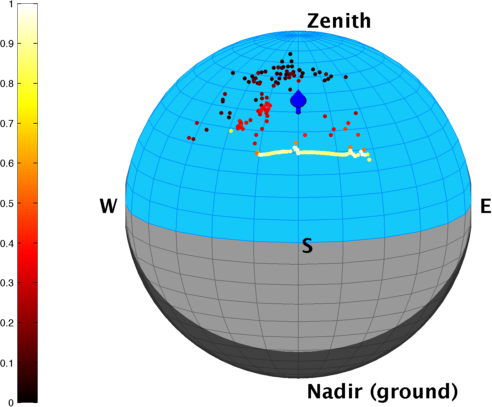
\includegraphics[height=1.43in]{sphereShift20131106_n1} \ \ %\\[3mm]
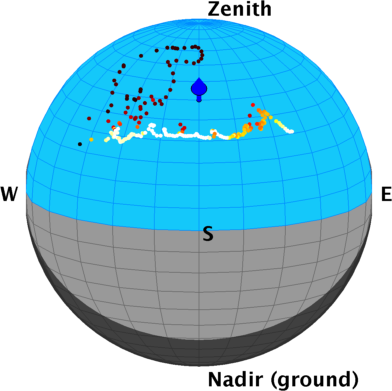
\includegraphics[height=1.43in]{sphereShift20141011_n1} \\[3mm]
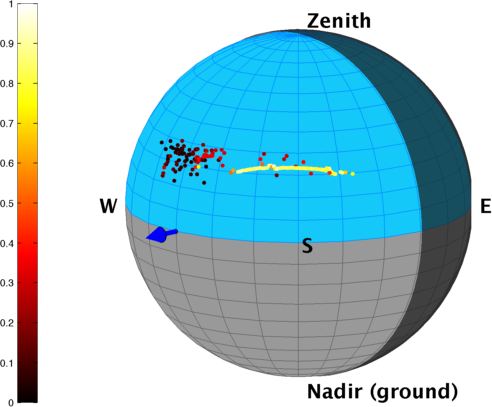
\includegraphics[height=1.43in]{sphereShift20131106_n2} \ \ %\\[3mm]
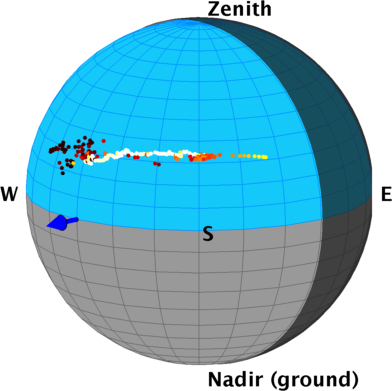
\includegraphics[height=1.43in]{sphereShift20141011_n2} \\[3mm]
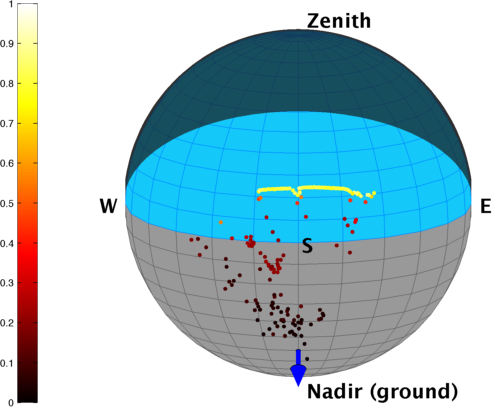
\includegraphics[height=1.43in]{sphereShift20131106_n3} \ \ %\\[3mm]
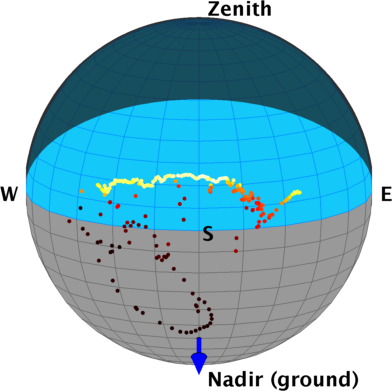
\includegraphics[height=1.43in]{sphereShift20141011_n3} \\[2mm]
{\footnotesize {\verb| |} \hspace{0.5cm} (a) Mixed clouds (06-NOV-13) \hspace{0.25cm} (b) Mixed clouds (11-OCT-14) }\\
\vspace{-2mm}
\caption{Globes representing the coordinate system of sky probes. Each normal (blue arrow) defines a shaded hemisphere in the environmental map that does not contribute light to the computed MLVs (dots). All MLVs in two particular partly cloudy days (columns) were computed from real environment maps~\cite{holdgeoffroy-iccp-15} for 3 example normal vectors (rows). Relative MLV intensities are shown in the color bar on the left. See also video in~\cite{webpageXhourPS}.}
\label{fig:realShiftNormal}
\vspace{-3mm}
\end{figure}%
% -----------------------------------------------------------------------------
% -----------------------------------------------------------------------------
\begin{figure}[!ht]
\centering
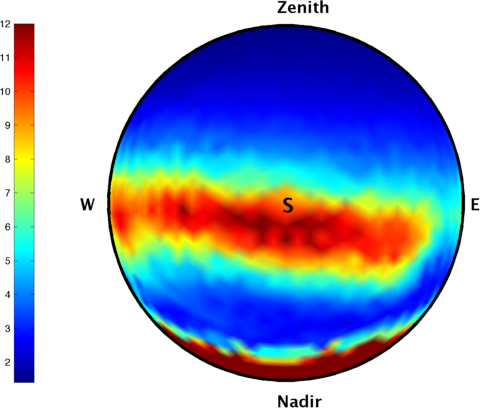
\includegraphics[height=1.46in]{sphereGain20131106} \ \ \ %\\[3mm]
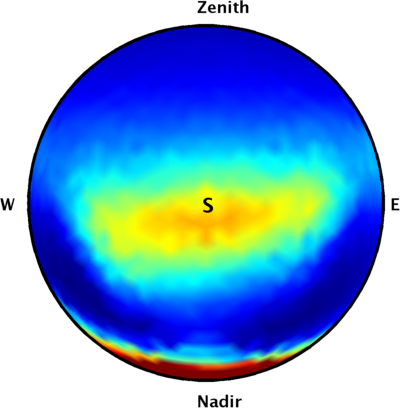
\includegraphics[height=1.46in]{sphereGain20141011} %\\[1mm]
{\footnotesize {\verb| |} \hspace{.6cm} (a) 06-NOV-13 \hspace{1cm} (b) 11-OCT-14 }\\[3mm]
\vspace{-2mm}
\caption{Noise gain for each normal direction ${\bf n}$ visible to the camera; the colors indicate the shifting (coplanarity) of the associated MLVs. The camera is assumed to lie to the South of this hypothetical target object. For both days, normals that are nearly horizontal are associated with more coplanar MLVs (smaller shifts, higher gains). These normals define a {\em zero-crossing region} between positive and negative out-of-plane shifts (mid row in fig.~\ref{fig:realShiftNormal}), where occlusion of the sun results in shifts that are predominantly {\em along} the solar arc. See also video available in~\cite{webpageXhourPS}.}
\label{fig:realShiftAll}
\vspace{-3mm}
\end{figure}
% -----------------------------------------------------------------------------


\subsubsection{Evolution of noise gain over time}

In this section, we show how the conditioning of outdoor PS evolves over time. Analyzing the patterns in its evolution will allow us to isolate important ``events''---points at which uncertainty suddenly drops---and investigate whether such events occur in close succession.

The main results are given in fig.~\ref{fig:events}, which plots the gain factor $\lambda_{\max}$ for all possible time intervals in four different days. Since $\lambda_{\max}$ varies with ${\bf n}$, we plot the median gain over 321 normal vectors visible to the camera (by subdividing an icosahedron three times) for each time interval.

The first row of fig.~\ref{fig:events}(a,b) illustrates the case of two days identified in sec.~\ref{subsec:mlv-clouds} as yielding poor outdoor PS reconstructions. As seen in the plots, low noise gains are never reached, irrespective of the start time and duration of the capture interval. We note that the (nearly) overcast sky of fig.~\ref{fig:events}(b) exhibits better behavior than the completely clear sky of fig.~\ref{fig:events}(a). This is because that day is not completely overcast, and the sun sometimes becomes visible (see the sun log-intensity plot). MLVs are thus shifted away from their main axes, while improving conditioning only slightly.

More interesting scenarios arise on days exhibiting a better mix of sun and moving clouds, such as the two examples in fig.~\ref{fig:events}(c,d). The two black vertical lines in fig.~\ref{fig:events}(c) identify capture intervals starting at two different times. Following the line labeled ``start time 1'' (beginning at 11:00), we notice that uncertainty remains high for approximately two hours, then suddenly drops at around 13:00. This time instant is followed by sudden changes in sun intensity (due to passing clouds) that are sufficient to shift the MLV away from the sun plane. Subsequently, uncertainty continues to decrease, albeit at a much slower pace, over the rest of the day. The second time interval (identified as ``start time 2'') starts at 14:00, so it does not benefit from that period of sun intensity changes. The maximum gain at the end of the interval is therefore higher. 

Of course, this could be due to a simple fact: the first interval is longer than the second one. However, fig.~\ref{fig:events}(d) shows that longer intervals do not always result in lower uncertainty. This time, two 2-hour intervals are considered. The time interval labeled as ``start time 1'' stops right before the 14:00 mark, and only sees clear skies; as expected, the uncertainty is very high. ``Start time 2'', beginning at 13:30, can fully exploit the MLV shifts caused by moving clouds to dramatically decrease PS uncertainty, even while the interval length is kept constant.
  
\begin{figure*}[!th]
\centering
\footnotesize
\setlength{\tabcolsep}{0pt}
\begin{tabular}{cc}
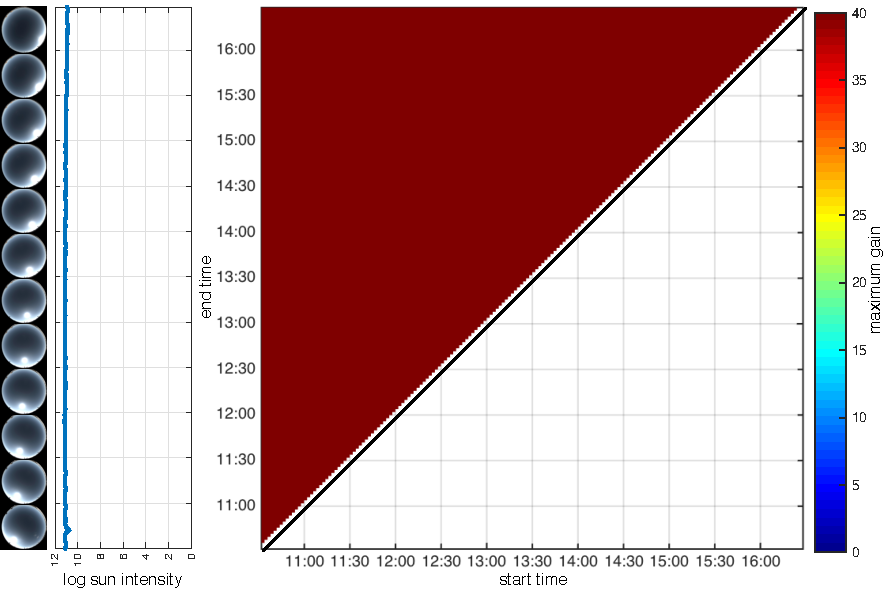
\includegraphics[height=5.7cm]{./figures/events/events-20141003-colorbar.pdf} & 
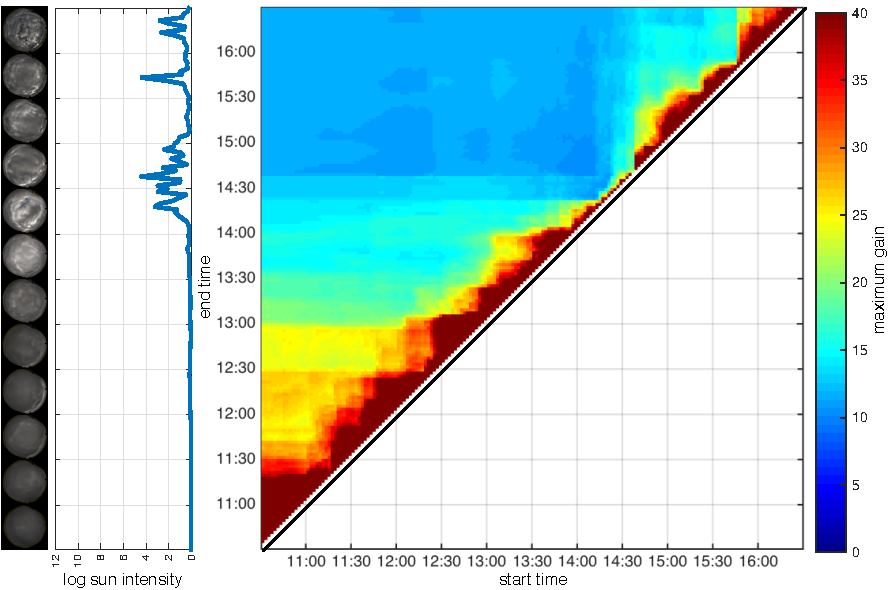
\includegraphics[height=5.7cm]{./figures/events/events-20131119-colorbar.pdf} \\
(a) Clear day (03-OCT-14) & (b) Nearly overcast day (19-NOV-13) \\%*[.5em]
% \multicolumn{2}{c}{\includegraphics[width=.3\linewidth]{./figures/events/colorbar-horizontal-withlegend.pdf}} \\%*[.5em]
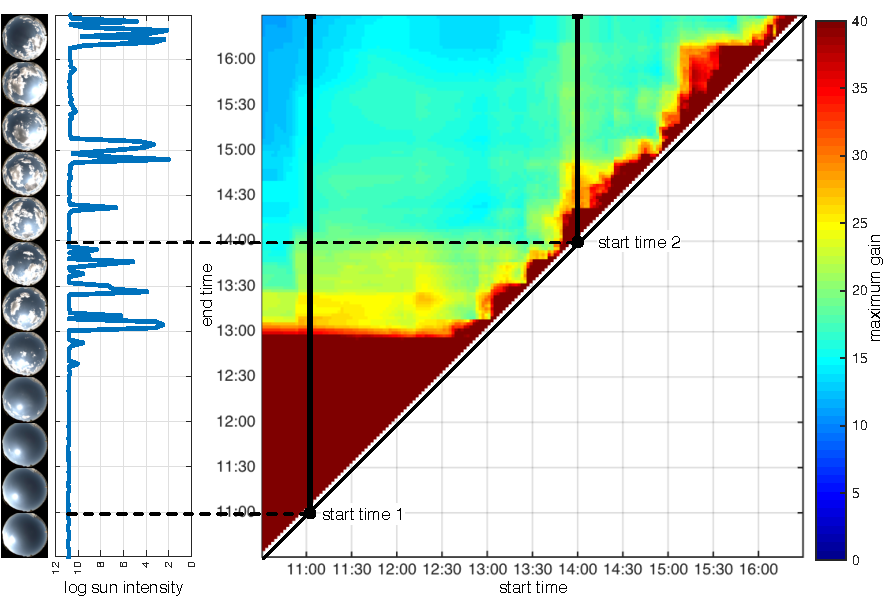
\includegraphics[height=5.7cm]{./figures/events/events-20130824-colorbar.pdf} & 
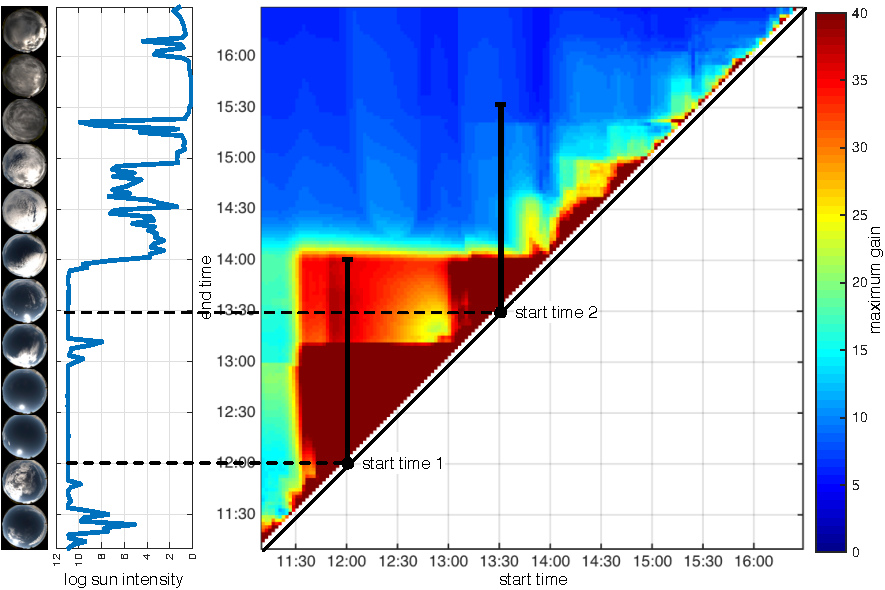
\includegraphics[height=5.7cm]{./figures/events/events-20131106-colorbar.pdf} \\
(c) Clear sky and mixed clouds (24-AUG-13) & (d) Mixed clouds (06-NOV-13)
\end{tabular}
\vspace{.25em}
\caption{Fine-grained analysis of the expected uncertainty of outdoor PS as a function of time over four selected days in the dataset. Colored plots show the maximum gain $\lambda_\text{max}$ as a function of start time (diagonal along the plot), and duration of the interval. The black lines identify particular time intervals discussed in the text. The blue curve to the left of each colored plot represents the log sun intensity over the course of that day. Photographs of the sky for each day are also shown on the left.}
\label{fig:events}
\end{figure*}

\subsubsection{Overall performance of $x$-hour PS}  

We noted in fig.~\ref{fig:events}(d) that sufficient conditions for low uncertainty could be met in as little as 2 hours. In this section, we evaluate how often one can achieve low uncertainty in short time intervals. This is done by assessing the distribution of noise gains from short time intervals, and aggregating results over multiple days.

To compute these statistics, we first consider a single normal and a single day. For a particular time interval \mbox{$\tau = \{t_\text{start}, t_\text{end}\}$}, we compute the ratio $r_\lambda(\tau)$ of its noise gain divided by the best (minimum) gain of all possible intervals in this day (including the full-day interval). Fig.~\ref{fig:ratios}(a,b) shows distributions of relative gains $r_\lambda$ for the two days in fig.~\ref{fig:events}(c,d). Fig.~\ref{fig:ratios}(a) shows that, for intervals of 4 hours, 75\% of the normals have uncertainty below twice the minimum gain for that day. In the case of fig.~\ref{fig:ratios}(b), that interval drops to 3 hours. 

The ratios $r_\lambda$ were then computed for all normals, over all days in the database. The compound statistics are shown in fig.~\ref{fig:ratios}(c). They empirically illustrate that there were many opportunities for stable normal reconstruction with short capture intervals. For example, more than 50\% of the time intervals of 3 hours resulted in reconstructions that had at most twice the uncertainty of the optimal interval. These results suggest that opportunities for shorter capture sessions seem to occur quite frequently in practice.

\begin{figure*}
    \footnotesize
    \centering
    \begin{tabular}{ccc}
    \setlength{\tabcolsep}{0pt}
    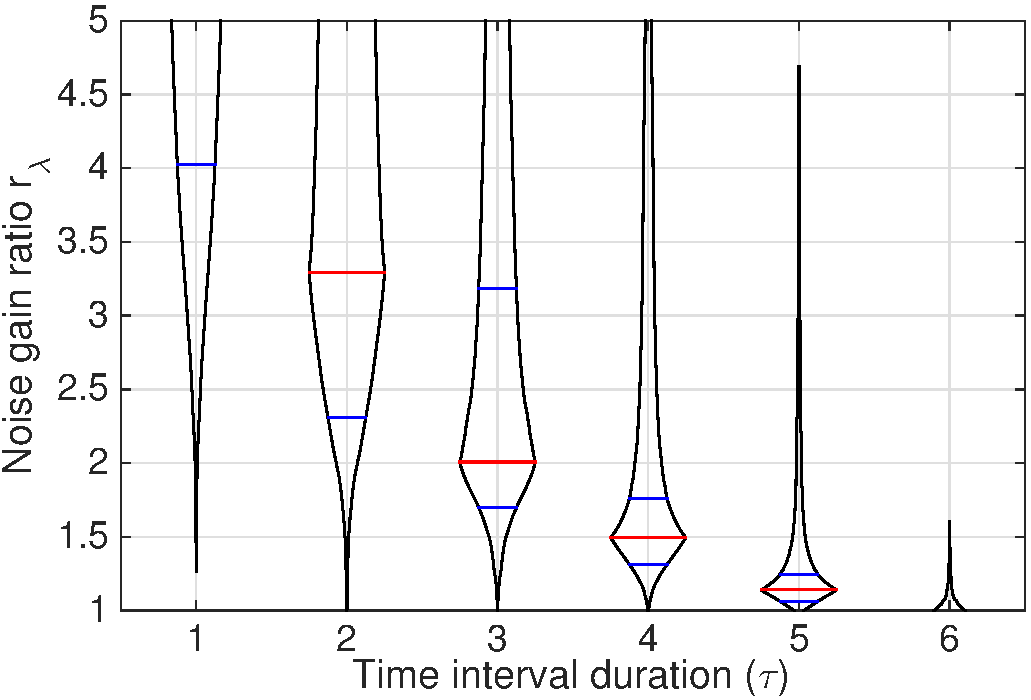
\includegraphics[width=.30\linewidth]{./figures/relativePerf/20130824-maxGain-global-relativePerf.pdf} & 
    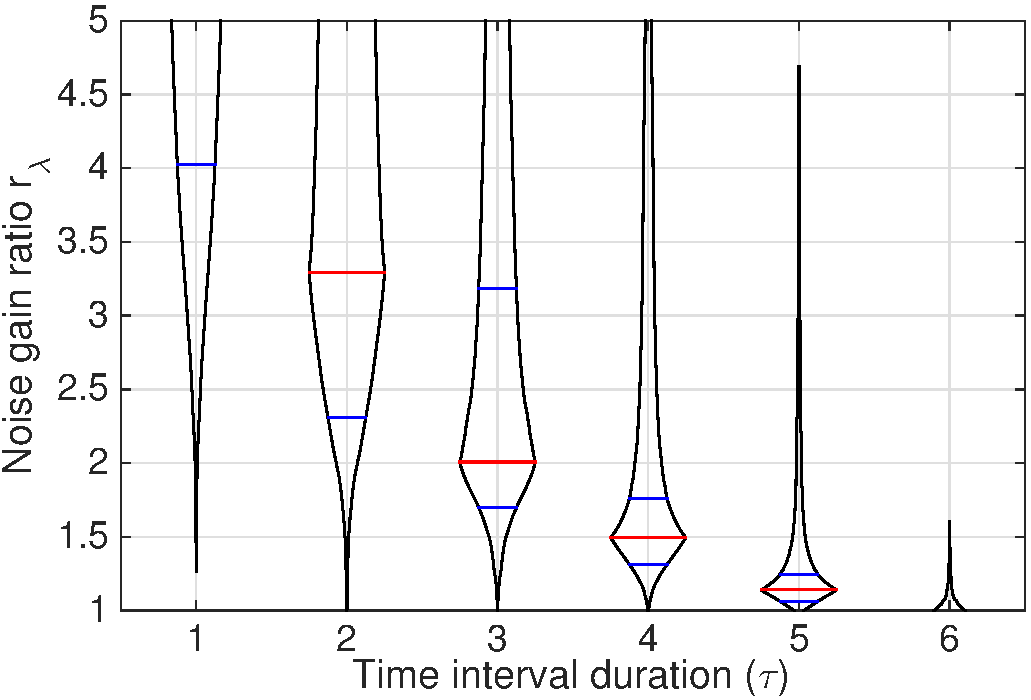
\includegraphics[width=.30\linewidth]{./figures/relativePerf/20130824-maxGain-global-relativePerf.pdf} & 
    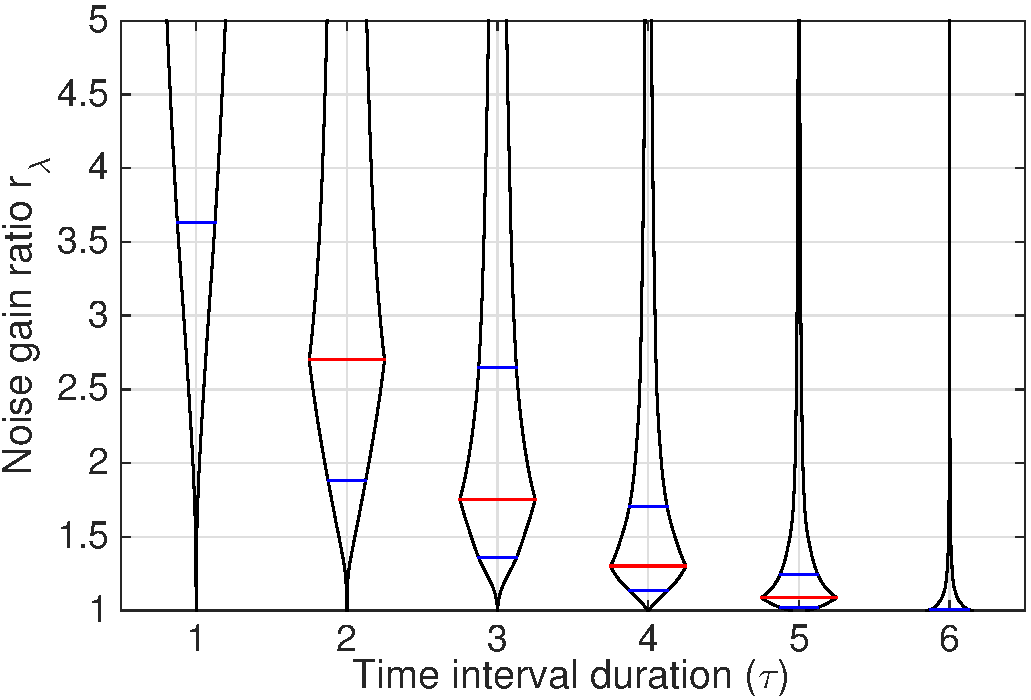
\includegraphics[width=.30\linewidth]{./figures/relativePerf/all-maxGain-relativePerf.pdf} \\
    (a) 24-AUG-13 & (b) 06-NOV-13 & (c) Entire dataset
    \end{tabular}
    \vspace{.15em}
    \caption[]{Distribution of noise gain ratio $r_\lambda(\tau)$ as a function of time interval duration: (a,b) two days in fig.~\ref{fig:events}; (c) across all the dataset. The~distributions of computed ratios are displayed vertically as ``box-percentile plots''~\cite{esty2003box}; the red horizontal bars indicate the median, while the bottom (top) blue bars are the 25th (75th) percentiles. }
    % THIS IS CONFUSING, DOESN'T HELP MUCH:
    %Note that durations include all intervals within $\pm 30\text{m}$ of the value indicated. For example, a duration of 4h includes all time intervals in the range $[3\text{h}30, 4\text{h}30]$.
    \label{fig:ratios}
\end{figure*}

%\begin{figure}
%\centering 
%\footnotesize
%\setlength{\tabcolsep}{0pt}
%\begin{tabular}{cc}
%\includegraphics[width=.49\linewidth]{./figures/relativePerf/20130824-cn-local-relativePerf.pdf} & 
%\includegraphics[width=.49\linewidth]{./figures/relativePerf/20131106-cn-local-relativePerf.pdf} \\
%(a) 24-AUG-13 & (b) 06-NOV-13
%\end{tabular} 
%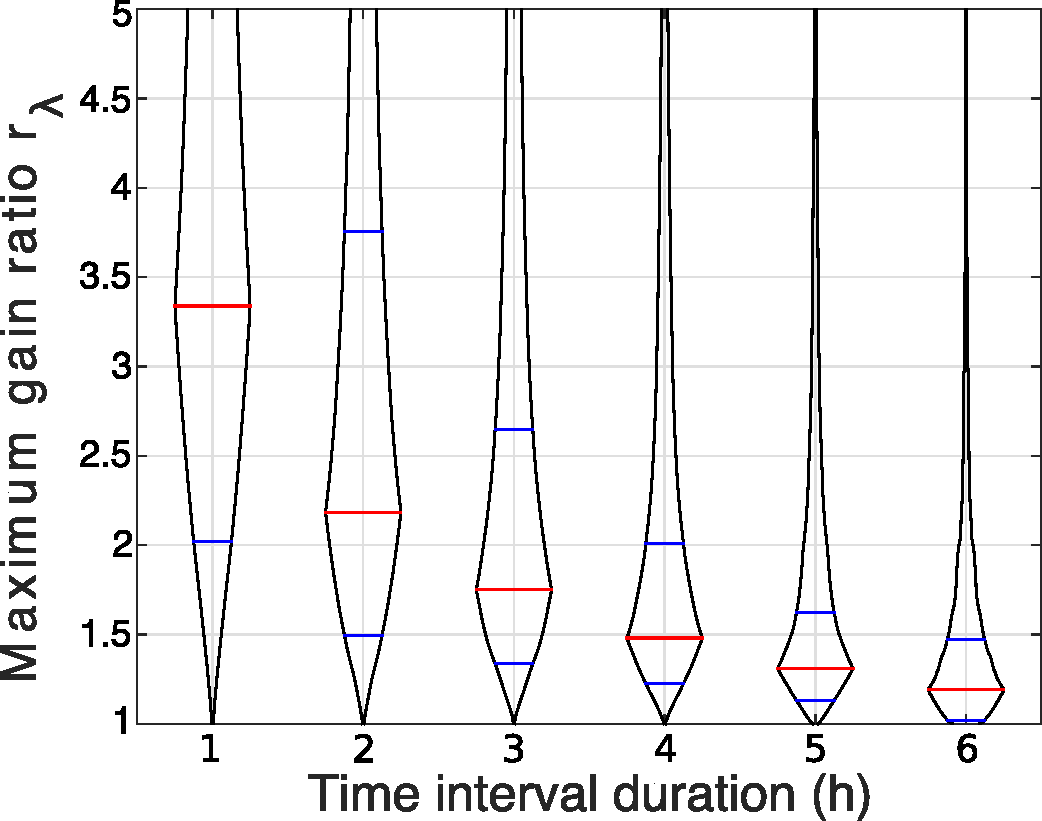
\includegraphics[width=.49\linewidth]{./figures/relativePerf/all-cn-relativePerf.pdf} \\
%(c) Entire dataset
%\vspace{.25em}
%\caption[]{Distribution of condition number ratio $r_t$ as a function of time interval duration, shown for (a,b) the same days as fig.~\ref{fig:events}, and (c) across the entire dataset. To display this ratio, we use ``box-percentile plots''~\cite{esty2003box}, which illustrate the distribution of ratios vertically. The red horizontal bars indicate the median, while the bottom (top) blue bars are the 25th (75th) percentiles. The outliers, illustrated by the long vertical tails above the 75th percentile, are due to normals pointing downwards, for which the expected uncertainty always remains high. Note that durations include all intervals withing $\pm 30\text{m}$ of the value indicated. For example, a duration of 4h includes all time intervals in the range $[3\text{h}30, 4\text{h}30]$. }
%\label{fig:ratios}
%\end{figure}


\begin{figure*}[t]
    \centering
    \footnotesize
    \begin{tabular}{cc}
        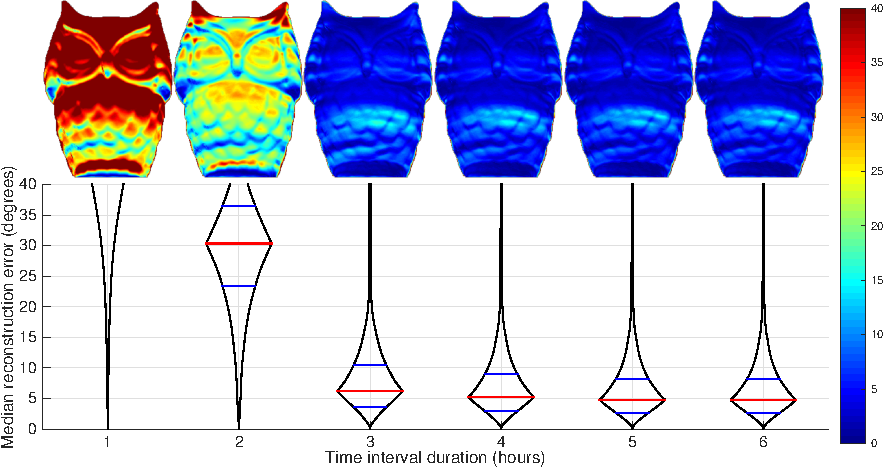
\includegraphics[height=5.7cm]{./figures/owl/owl-12h.pdf} & 
        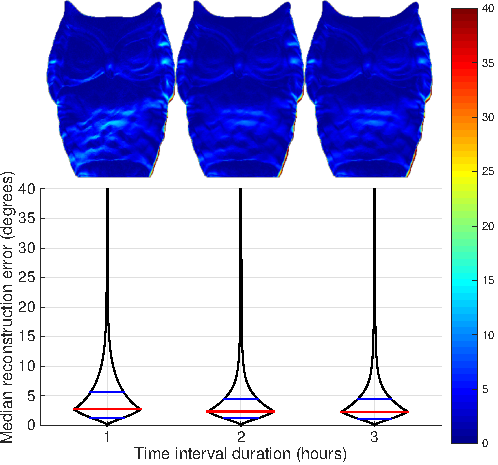
\includegraphics[height=5.7cm]{./figures/owl/owl-13h30.pdf} \\
        (a) Intervals starting at 12:00 on 06-NOV-13 & (b) Intervals starting at 13:30 on 06-NOV-13
    \end{tabular}
    \vspace{1mm}
    \caption{Normal recovery error as a function of time interval and start time: (a) 12h00 and (b) 13h30 on 06-NOV-13. Experiments are performed on a synthetic object rendered with real sky probes and additive Gaussian noise $\sigma=1\%$. The top row shows per-pixel angular error, color-coded as in the scale on the right. The bottom row shows box-percentile error plots (see fig.~\ref{fig:ratios}). As suggested in fig.~\ref{fig:events}(d), the performances of \{3,4,5,6\}-hour outdoor PS are very similar (a). Even 1-hour outdoor PS can be competitive if started at the right time (b).}
    \label{fig:owl-results}
    \vspace{-3mm}
\end{figure*}

\begin{figure}[!t]
    \centering
    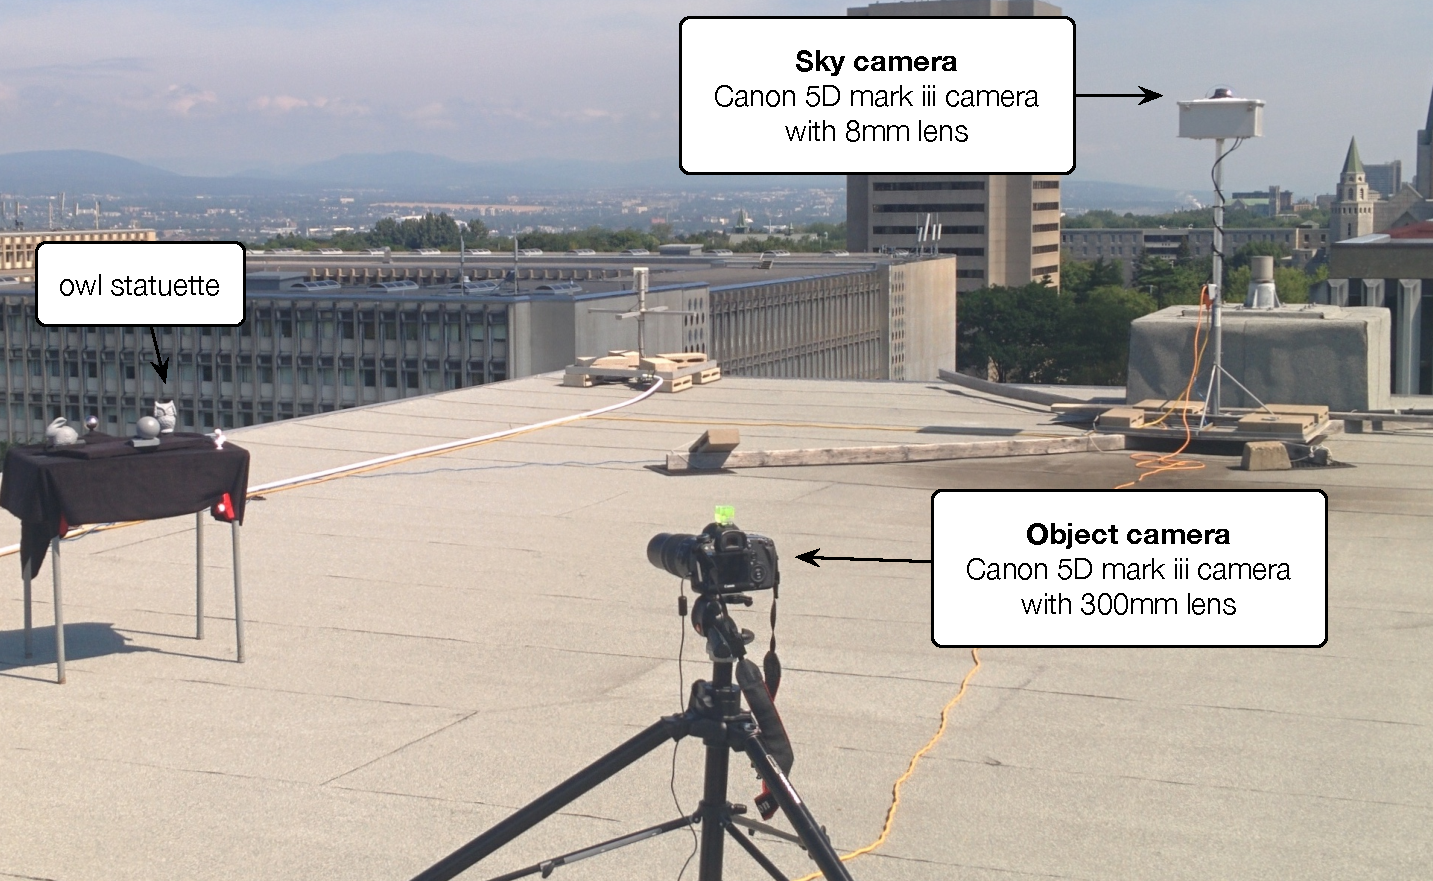
\includegraphics[width=.92\linewidth]{./figures/realData/realData-setup.pdf} \\[1mm]
    \caption{Real data capture setup. HDR photographs of the sky and of the object (owl statuette) are simultaneously captured by two cameras installed on the roof of a tall building.}
    \label{fig:real-data-setup}
    \vspace{-2mm}
\end{figure}

\begin{figure*}[t]
    \centering
    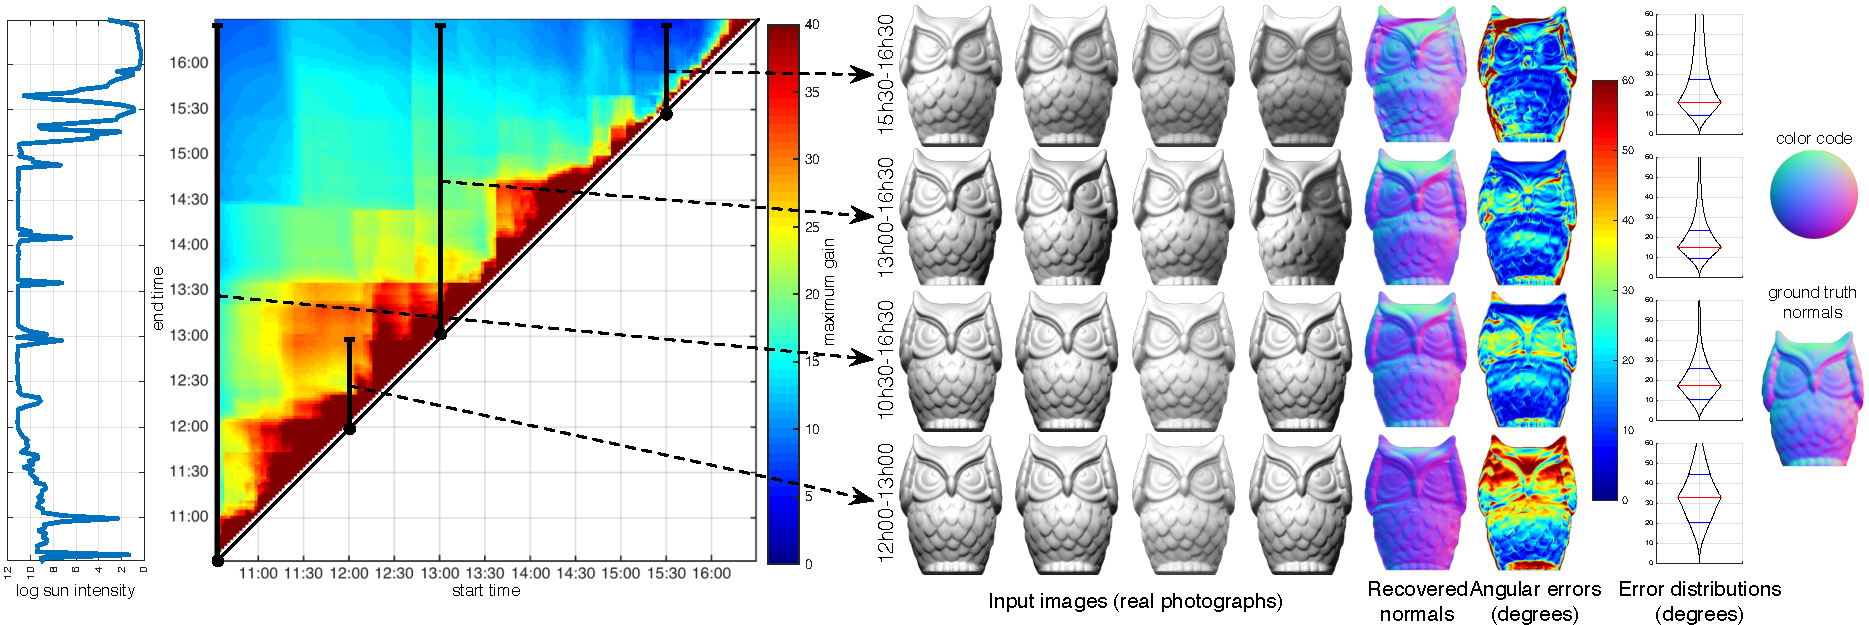
\includegraphics[width=\linewidth]{./figures/realData/realData4.pdf}
    \caption{Validation on real data, captured on 11-OCT-14 (partly cloudy). Four distinct time intervals are analyzed and, for each one, the following information is displayed, from left to right: ($i$) log sun intensity; ($ii$) noise gain $\lambda_\text{max}$ as a function of start time and duration of the interval, as in fig.~\ref{fig:events}; ($iii$) example input images; ($iv$) normals recovered by calibrated outdoor PS; ($v$) normal estimation error at each pixel; and ($vi$) the error distribution, in degrees. For reference, ground truth normals are given on the rightmost plots.}
    \label{fig:real-results}
    \vspace{-2mm}
\end{figure*}

\subsection{Experimental validation}

We validate the analyses in sec.~\ref{sec:sensitivity-analysis} and \ref{sec:analysis} via calibrated outdoor PS on synthetic and real object images with known ground truth normals. These normals are used as an optimal initialization for computing ground-truth MLVs, thus avoiding convergence issues of nonlinear optimization and allowing us to focus on assessing errors due to illumination effects in the real sky probes. We then perform calibrated outdoor PS on these images using the algorithm in \cite{yu-iccp-13}, with the following two differences: (\emph{i}) we use all possible pairs of images to compute ratios, instead of selecting a single denominator image; and (\emph{ii}) we apply anisotropic regularization~\cite{hernandez-pami-11} to mitigate the impact of badly-conditioned pixels on the surface reconstruction.

%
\vspace{-3mm}
\paragraph{Synthetic data}%
%
We first consider synthetic images of an owl model rendered with real sky probes. The rendered images were perturbed with additive Gaussian noise at 1\% the median pixel intensity. For each image, one real-world environment map from the database was used as the sole light source. Cast shadows were not simulated to isolate the analysis to the photometric cue alone (see~\cite{webpageXhourPS} for more realistic results with a physically-based rendering engine). 

% \begin{figure}
% \centering
% \newlength{\mylength}
% \setlength{\mylength}{.19\linewidth}
% \todo{Replace with renderings with luxrender... }
% \caption{Example renderings of the owl model used in the validation experiments for 06-NOV-13 (see figs~\ref{fig:events}, \ref{fig:owl-results}). Images are tone-mapped for display ($\gamma=1.8$).}
% \label{fig:owl-synthetic-data}
% \vspace{.5em} 
% \end{figure}

We ran calibrated outdoor PS on all time intervals starting at 12:00 or 13:30 for the day 06-NOV-13 (see fig.~\ref{fig:events}(d)), in increments of one hour. The main results of this experiment are shown in fig.~\ref{fig:owl-results}. Fig.~\ref{fig:owl-results}(a) follows ``start time 1'' in fig.~\ref{fig:events}(d); the reconstruction error improves significantly until an interval of 3 hours is reached, at which point the error improves only slightly through the rest of the day. Thus, the additional data provides little new information. In fig.~\ref{fig:owl-results}(b), we now follow the path of ``start time 2'' in fig.~\ref{fig:events}(d); in this case, the error is already quite low after just one hour.
%
\vspace{-3mm}
\paragraph{Real data}%
%
Another similar experiment considered real photos of a real owl statuette. To capture this data, we set up two cameras on the roof of a tall building as shown in fig.~\ref{fig:real-data-setup}. The first camera, dubbed ``sky camera'', captures omnidirectional photos of the sky using the approach proposed by Stumpfel \etal~\cite{stumpfel-afrigraph-04}. The second, ``object'' camera is equipped with a telephoto zoom lens and captures photos of the statuette. Both cameras capture exposure-bracketed HDR photos simultaneously, once every two minutes\footnote{Data and source code are available on our project webpage~\cite{webpageXhourPS}.}. Ground truth surface normals were obtained by aligning a 3D model of the object (obtained with a 3D scanner) to the image using POSIT~\cite{dementhon1995model}. 

The validation results with real data are shown in fig.~\ref{fig:real-results}. As predicted by the noise gain values of fig.~\ref{fig:real-results}~(left), similar reconstruction performance is obtained from three different time intervals shown in the top three rows of fig.~\ref{fig:real-results}~(right). Once again, the performances of 1-hour (15:30--16:30) and 3.5-hour (13:00--16:30) outdoor PS are indeed quite close to that of ``full-day'' outdoor PS (10:30--16:30). However, not all one-hour intervals are equally good, as shown for the interval 12:00--13:00 at the bottom of fig.~\ref{fig:real-results}.


\subsubsection{Discussion}
\label{sec:3dv-discussion}

In this paper, we present what we believe is the first study of the time requirements for single-day outdoor PS. In particular, we seek to determine the relationship between expected performance in normal estimation and: (\emph{i}) the duration of data capture within a single, arbitrary day; and (\emph{ii}) specific atmospheric events that introduce beneficial lighting variations during that time interval. To achieve this goal, we use a large database of natural, outdoor illumination (sky probes) and take a detailed look at the conditions under which surface normals can be reconstructed reliably. \mbox{Finally,} we investigate whether these conditions are observed in less than a full day of data capture.

Our analysis reveals the following novel insights. First, we show how the mean light vectors (MLVs) are shifted from the solar plane when the sun is occluded by clouds. We demonstrate, through an extensive empirical analysis, that the atmospheric events causing that shift occur often in practice, and that they can be observed within a short time interval. In addition, we found that this shifting is often sufficient to constrain the PS problem significantly and reduce uncertainty in normal estimation. However, we also show that the shift is not the same for every normal; for some normals, shifting may not reduce uncertainty sufficiently. Finally, we validate our analysis by running calibrated outdoor PS on synthetic and real data. 

One limitation of our work is that we consider only contiguous time intervals. It would be interesting to explore how non-consecutive images could be selected, from a given interval, with the goal of achieving additional improvements in performance. Presently, we are using the setup in fig.~\ref{fig:real-data-setup} to collect a database of real objects observed outdoors, and extending our analysis considering more elaborate shading and ground models.

We believe our findings open the way for interesting new research problems. Of note, one could leverage knowledge on MLV shifting to steer regularization in outdoor PS and even attempt to further reduce time requirements. It would also be interesting to include other cues, such as shape priors or stereo, to further constrain the problem. We plan to explore these issues in future work.

% What we have analyzed...

% Summary of main findings...

% These are only relative predictions and, ultimately, absolute performance depends on the actual sensor noise (baseline uncertainty) and surface reflectance (albedo). 

% Normals nearly horizontal present MLVs that are closer to being coplanar, why? Interesting direction for future research.

% For both days, normals that are nearly horizontal are associated with more coplanar MLVs (smaller shifting). This is also visible in the second row of fig.~\ref{fig:realShiftNormal}. This is observed because those normals represent the point at which the intensities coming from the top half of the normal hemisphere is similar to those coming from the bottom half. Occluding the sun therefore does not result in a significant shift in the dominant light direction.
 
% Uncertainty is higher, more errors, suggest direction for future investigation on regularization methods.

% % Maybe we can include this to emphasize the important of our results here

% The results presented here are very important as reducing the time interval for PS reconstruction can open the way for capturing non-static outdoor objects that present some small amount of dynamics. We believe this to be an exciting new direction for future research.


